\documentclass{subfiles}
\begin{document}
\section{Quantum Mechanics}
\subsection*{The quantum mechanical wavefunction and the Schrödinger Equation}
The physical description of any quantum system, i.e the \emph{state space}, is given by the quantum mechanical \emph{wavefunction} (also often called a \emph{state vector})\cite{nielsen2010quantum}, which in Dirac notation\footnote{Named after the physicist Paul Dirac, who was one of the founding fathers of quantum mechanics.} is written as $\ket{\Psi(t)}$. 
This function is a complex-valued function that gives a complete description of both static and dynamic properties of a given quantum system, and thus presents the analogue to the classical notion of a set of trajectories in phase space \cite{hochstuhl2014time}. 

The dynamics of the wavefunction is governed by the \emph{Time-dependent Schrödinger Equation} (TDSE),
\begin{equation}
    i\frac{\partial}{\partial t}\ket{\Psi(x, t)} = H(x,t)\ket{\Psi(x, t)}\label{eq:_tdse}
\end{equation}
where $H$ a linear hermitian operator often referred to as the \emph{Hamiltonian}. Here $x$ is the position of the particle, and $t$ is the time. 
This operator describes the total energy of the system, and is given by (in atomic units) \textcolor{red}{(Add more about the Hamiltonian, also see chapter 2.1.1 in Szabo Ostlund for material on atomic units. This is probably needed for results (to have proper discussions, and a real sense of "distance" in the results section). In the book, atomic units are as follows: length $=0.52918$ (Å), energy $=27.211$ (eV), dipole-moment (two charges at distance $a_0$) $=2.5418$ Debyes (D). There is also a conversion table that could prove useful.)}
\begin{align*}
    H = -\nabla^2 + V(\mathbf{r})
\end{align*}
where $\nabla^2$ is the Laplacian operator, and $V(\mathbf{r})$ is the potential energy of the system, both external and internal.


This equation gives the equation of motion for the wavefunction, and describes how the wavefunction evolves in time.
\subsection*{Second Quantization}
As the earliest formulations of quantum mechanics introduced the ground-breaking concepts of quantized properties like energy, momentum and angular momentum, we can think of this formulation as a "first quantization". Here the observables are represented as operators with real eigenvalues and wavefunctions are assigned to individual particles.
As quantum mechanics matured, it became clear that first quantization was not sufficient to describe many-body systems - especially systems with indistinguishable particles, such as fermionic structures, or systems where particles are created or annihilated, such as in chemical reactions, or in the study of elementary particles.\\  
Second quantization solves this problem by introducing a new mathematical framework, which accounts for both the particle indistinguishability and the creation and annihilation of particles, and makes the statefunction also expressed in terms of operators. Furthermore, second quantization allows for a more intuitive and compact notation for many-body systems, where instead of asking "where is particle $i$?", we ask "how many particles are in \emph{state} $i$?". 
As such, second quantization is often referred to as the "occupation number representation" of quantum mechanics. This moves the focus from the individual particles to the orbitals they occupy. This reformulation also reduces much of the manipulation of the wavefunction to algebraic operations, which makes numerical implementations much more efficient, and easy to understand.\cite{helgaker2013molecular}.
\\ \\ In second quantization, we introduce a set of creation and annihilation operators, $a^\dagger$ and $a$, which create and annihilate particles in a given state. An important thing to note, is that these operators differ depending on the type of particles. For bosons, these operators satisfy the following commutation relations:
\begin{align}
    [a_i, a_j] = [a^\dagger_i, a^\dagger_j] = 0, \quad [a_i, a^\dagger_j] = \delta_{ij}\label{eq:commutation}
\end{align}
where $[A, B] = AB - BA$, and for fermions, the \emph{anti-}commutation relations are:
\begin{align}
    \{a_i, a_j\} = \{a^\dagger_i, a^\dagger_j\} = 0, \quad \{a_i, a^\dagger_j\} = \delta_{ij}\label{eq:anti_commutation}
\end{align}
where $\{A, B\} = AB + BA$.
\subsection{Fock Space}
In the framework of second quantization, the concept of a \emph{Fock space}\footnote{First introduced by V. A. Fock in \cite{fock1932konfigurationsraum}} emerge naturally as a mathematical structure for describing quantum systems with variable, or uknown, number of particles. A Fock space is a direct sum of Hilbert spaces, 
\begin{align*}
    \mathcal{F} = \bigotimes_{n=0}^\infty S_{\pm} \mathcal{H}_n
\end{align*}
where each space, $\mathcal{H}_n$ represents a state with fixed a number of particles, and $S_{\pm}$ is the symmetrization operator for bosons ($+$) and fermions ($-$). Meaning, the zero-particle states, one-particle states, two-particle states etc. This encapsulates all possible configurations of a many-body system elegantly. Using the occupation number representation introduced in second quantization, a state in Fock space is not expressed by momenta or position, but rather by the number of particles occupying certain quantum states. \\
For instance, the state $\ket{n_1, n_2, ...}$ informs that $n_1$ particles occupy state $1$, $n_2$ particles  in state $2$. The annihilation and creation operators act on the Fock states by increasing, or decreasing, the occupation numbers of the corresponding states. E.g. the action of the creation operator on a state is given by
\begin{align*}
    a^\dagger_i\ket{n_1, n_2, ...} = \sqrt{n_i + 1}\ket{n_1, n_2, ..., n_i + 1, ...}.
\end{align*}
From this, these operators can describe particle interactions, transitions and dynamics in a many-body system. As the Fock space is constructed by direct sums, two states of different particle numbers are inherently orthogonal 
\\\\ 
For systems of indistinguishable particles, Fock spaces naturally incorporate the Pauli exclusion principle, as the anti-commutation relations \ref{eq:anti_commutation} ensure that no two fermions can occupy the same quantum state. This fundamental property of fermions explains, for example, why electrons in an atom cannot share identical quantum numbers. For bosonic systems (distinguishable particles), the commutation relations \ref{eq:commutation} instead allow multiple particles to occupy the same state, which is crucial for phenomena such as Bose-Einstein condensation.
\subsection*{Hartree-Fock}\label{sec:HF_theory}
Accurately solving the Schödinger equation for many-body systems is a formidable challenge, even in seemingly simple cases such as a one-dimensional system with few interacting, indistinguishable particles. The inherent complexity arise from the interactions between particles, the Pauli exclusion principle, and the indistinguishability of particles. As we mentioned in the section on Hilbert spaces\ref{sec:Hilbert_space}, the dimension of the Hilbert space grows exponentially with the number of particles, making exact solutions computationally infeasible. In many cases, such a molecular dynamics and solid-state physics, the Hilbert space is reduced dramatically by imposing the Born-Oppenheimer approximation, which separates the electronic and nuclear motion, effectively disregarding the degrees of freedom of the nuclei by treating the nuclei as fixed. Even so, the many-body problem remains an intractable problem for classical computers, and finding approximate solutions to the Schrödinger equation is therefore necessary. The \emph{Hartree-Fock} method is a fundamental approach for solving the many-body problem in quantum chemistry. In this section, we will examine the theory behind the method in detail, beginning with essential concepts from quantum many-body theory, setting the stage for the method to be presented in later sections. \\ \\

%% Many-body concepts
In any many-electron system, the indistinguishability of particles introduce a fundamental contraint on the wavefunction, namely that is must be anti-symmetric under the exchange of any two particles. i.e 
\begin{align*}
    \Psi(\mathbf{r}_1, \mathbf{r}_2, ..., \mathbf{r}_N) = -\Psi(\mathbf{r}_2, \mathbf{r}_1, ..., \mathbf{r}_N)
\end{align*}
This constraint is known as the \emph{Pauli exclusion principle}, which require that no two electrons can occupy the same quantum state. A common way to incorporate this mathematically is to construct wavefunctions using Slater determinants of single-particle orbitals (functions). These orbitals are our basis set of choice $\{\phi_i\}$, and a slater determinant is constructed as follows:
\begin{align*}
    \Psi(\mathbf{r}_1, \mathbf{r}_2, ..., \mathbf{r}_N) = \frac{1}{\sqrt{N!}}\begin{vmatrix}
        \phi_1(\mathbf{r}_1) & \phi_2(\mathbf{r}_1) & \cdots & \phi_N(\mathbf{r}_1)\\
        \phi_1(\mathbf{r}_2) & \phi_2(\mathbf{r}_2) & \cdots & \phi_N(\mathbf{r}_2)\\
        \vdots & \vdots & \ddots & \vdots\\
        \phi_1(\mathbf{r}_N) & \phi_2(\mathbf{r}_N) & \cdots & \phi_N(\mathbf{r}_N)
    \end{vmatrix}
\end{align*}
The mathematical nature of the determinant incorporates the anti-symmetry under particle exchange, as by swapping two columns in a determinant, the sign changes. The Slater determinant are a linear combination of \emph{Hartree products} built from the single-particle orbitals, which are products of spatial orbitals with (or without) the spin orbitals where the spin part is often omitted for simplicity. These single-particle orbitals are the solution of the one-electron Schrödinger equation, 
\begin{align*}
    \hat{h}\phi_i = \epsilon_i\phi_i
\end{align*}
where the full Hamiltonian (for a non-interacting) system would be 
\begin{align*}
    H = \sum_{i=1}^N \hat{h}_i
\end{align*}
which has the solution eigenvector
\begin{align}
    \Psi = \phi_1(\mathbf{r}_1)\phi_2(\mathbf{r}_2)...\phi_N(\mathbf{r}_N)\label{eq:hartree_product}
\end{align}
with corresponding eigenvalue $E = \epsilon_1 + \epsilon_2 + ... + \epsilon_N$, i.e. the sum of single-particle energies. Eq. \ref{eq:hartree_procut} is the Hartree product, and it is the simplest possible wavefunction for a many-body system of non-interacting particles. As is evident, this Hartree product is not anti-symmtric, nor indistinguishable, as the particles are designated a specific orbital to occupy and thus they are distinguishable, which is why the Slater determinant builds linear combinations of such products. In our study, we will make use of both - as our system can be constructed to both exhibit distinguishable and indistinguishable behaviour.\\ \\
Another important concept is the \emph{variational principle}, which states that, for any quantum system, the expectation value of the energy is always greater than, or equal to, the true ground state energy. 
\begin{align}
    E[\Psi] = \frac{\braket{\Psi|H|\Psi}}{\braket{\Psi|\Psi}} \geq E_0 \label{eq:variational_principle}
\end{align}
where $\Psi$ is the trial wavefunction, $H$ is the Hamiltonian operator, and $E_0$ is the true ground state energy of our system. The trial wavefunction in question could be a slater determinant, built from an initial guess for a "good" basis. As previously explained, we may transform this basis using unitary matrices to find a "better" basis, which in this case, would make our energy estimate \emph{lower}. This is the essence of the Hartree-Fock method, where we iteratively improve our basis set to minimize the energy of the system by use of the variational method. For more material and details on the variational method, we refer the reader to chapter 1.3 in \cite{szabo1996modern}.
\\\\
To arrive at the Hartree-Fock equations, we start at the variational principle
\begin{align*}
    E_0 \leq E^{HF} = \bra{\psi^{HF}}H\ket{\psi^{HF}}
\end{align*}
where $\ket{\psi^{HF}}$ is the Hartree-Fock wavefunction, which is a single Slater determinant, and it is normalized so we can omit the denominator in the expectation value. This basis is related to a chosen initial basis by a unitary transformation.
\begin{align*}
    \psi^{HF}_p = \sum_qC_{qp}\psi_q
\end{align*}
where the unitary matrix is expressed by its matrix elements. The Hamiltonian in question is the sum of the kinetic energy operator and the electron-electron repulsion operator, and the energy is given, expressed in the initial basis with the coefficients $C_p$, as
\begin{align*}
    E^{HF} = \sum_i\sum_{pq}C^*_{ip}C_{i}qh_{pq} + \frac{1}{2}\sum_{ij}\sum_{pqrs}C^*_{ip}C^*_{jq}C_{ir}C_{j}su_{pqrs}
\end{align*}
here expressed in terms of the one- and two-electron integrals, in the initial basis. The Hartree-Fock equations are derived by minimizing the energy with respect to the coefficients $C_{ip}$. We take the derivative w.r.t $C_{i}p^*$ which gives us the Hartree-Fock equations
\begin{align*}
    \sum_qh_{pq}C_{iq} + \sum_j\sum_{qrs}C^*_{jr}C_{js}u_{pqrs}C_{iq} = \epsilon^{HF}_{ip}C_{ip}.
\end{align*}
By assumption, the summation over $r$ and $s$ is over all the occupied orbitals (below the Fermi level), as these are the only ones that contribute in the (mean-field) interaction matrix. As a result, the indices reduce to a summation over the occupied orbitals only. This simplification modifies the two-body integrals into $u_{piqi}$, where $i$ runs over orbitals below the Fermi level, while $p,q$ remains the orbitals being varied. This simplification reflects the mean-field approximation central in Hartree-Fock theory, as only interactions with occupied orbitals are considereed. With this, we can now define the Fock operator as
\begin{align*}
    f_{pq} = h_{pq} + \sum_{i<F}C^*_{i}C_{i}u_{piqi}
\end{align*}
and the Hartree-Fock equations can be written as
\begin{align*}
    f_{pq}C_{iq} = \epsilon^{HF}_{ip}C_{ip}
\end{align*}
which is now a pseduo-eigenvalue equation that we need to solve iteratively. To solve this equation we employ the \emph{Self-Consistent Field} (SCF) procedure, an iterative method designed to converge to the ground-state energy of the system. This procedure starts with an initial guess for the coefficients $C_{ip}^{(0)}$, which defines the initial guess for the molecular orbitals. With this guess, the Fock operator is constructed, and the Hartree-Fock equations are solved. This yields a new set of coefficients $C_{ip}^{(1)}$, and the process is repeated until the HF-energies $\epsilon^{HF}$ converge within a set threshold, or the change in coefficients $C_{ip}$ becomes negligable. A more thorough presentation of the SCF method applied to the Hartree-Fock equations will be presented in later sections. \textcolor   

\textcolor{red}{Maybe add some more references. What about showing explicitly the integrals? Also the coulomb and exchange terms, maybe these would be good to show. SHould we talk about the Roothan-Hall equations?? No clue what that even is, but sounds cool perhaps. Also would be easier to cite.}

\begin{itemize}
    \item Born-Oppenheimer approximation, herein lies the separation of electronic and nuclear motion and mean-field approximation comes in naturally.
    \item Slater Determinants
    \item Hartree products
    \item Link in orbitals?
    \item Variational principle should be mentioned
    \item 
\end{itemize}

\subsection{Bipartite Hartree}
The Hartree-Fock method is a powerful tool for solving many-body quantum mechanical problems, but it makes an assumption that the wavefunction is described by a single Slater determinant, which represents anti-symmetric wavefunctions and thus indistinguishable particles. As explained in the previous section, our system is set up in such a way that our two-particle system behaves like distinguishable particles. Therefore, we may express our wavefunction as a \emph{Hartree product}, as we've explained in earlier sections. We can derive a similar procedure to find optimal basis transformations as in the section on Hartree-Fock. \\
The groundstate wavefunction will then have the following form:
\begin{align*}
    \ket{\Psi} = \ket{\phi^A_0\phi^B_0}
\end{align*}
where $\phi_0^M$ is the single-particle Hartree functions (orbitals) for subsystem $M\in[A,B]$, with the constraint that these single-particle orbitals are orthonormal. We can set up the Lagrangian
\begin{align*}
    L = E_H - \lambda^A(\braket{\phi^A_0|\phi^A_0} - 1) - \lambda^B(\braket{\phi^B_0|\phi^B_0} - 1)
\end{align*}
where $\lambda^M$ are the Lagrange multipliers, and $E_H$ is the Hartree energy, which is the expectation value of the Hamiltonian in the Hartree product state
\begin{align*}
    E_H = \bra{\Psi}H\ket{\Psi} = \bra{\phi^A_0}h^A\ket{\phi^A_0} + \bra{\phi^B_0}h^B\ket{\phi^B_0} + \braket{\phi^A_0\phi^B_0|u|\phi^A_0\phi^B_0}
\end{align*}
here $h^M$ are the single-body Hamiltonian, for each subsystem and $V$ the mean-field Coulomb interaction between subsystems. The Hartree orbitals can be expaneded in our single-particle basis set, as linear combinations, 
\begin{align*}
    \ket{\phi^M_i} = \sum_{\alpha=1}^{N^M} C^M_{\alpha i}\ket{\psi_\alpha}
\end{align*}
where $N^M$ is the number of single-particle basis functions in subsystem $M$. Minimizing the Lagrangian by the basis transformation cofficients $C_{\alpha i}^M$ gives us two coupled eigenvalue equations, i.e calculating $\frac{\partial L}{\partial C_{\alpha i}^M} = 0$ for $M\in[A,B]$, approximating the integrals by the quadrature rule \cite{leinonen2024coulomb}
\begin{align*}
    \bra{\psi_\alpha^M}h^M\ket{\psi_\beta^M} = \delta x \sum_i
\end{align*}



%%% MORSE  POTENTIAL
\subsection*{Morse potential}
To build our qubit system, we need to define some form of potential trap that we can confine our particles within. In modern quantum computing many different potentials are used, tested and theorized. One of the most common potentials are the quantum harmonic oscillator potential (QHO), a very well known potential in quantum mechanics. This potential has been studied in great detail and has been used in many different quantum systems, and is very often used as a benchmark for more advanced symmetric potentials. \textcolor{red}{(Cite some sources here)}. The QHO basis sets are widely employed to study quantum dot systems\cite{Yuan_2017}, and are often used in quantum chemistry to describe molecular vibrations. In our study, we will also employ the QHO potential to test our implementations and to compare our results with other studies.\textcolor{red}{will we?}
\\ \\ One could think that using the QHO potential for our qubit would be a natural choice, but there are some nuances necessary to consider. The QHO double well potential is perfectly symmetric, meaning the energy levels are uniformly spaced, and equal across both wells. This in not ideal for our realization of the iSwap gate, as we need more control over eneregy levels in both wells. \\ \\ To achieve this, we will instead use the Morsee potential, first introduced by Philip M. Morse in 1929 as a solution to the Schrödinger equation representing the motion of the nuclei in a diatomic molecule\cite{morse1929diatomic}. This potential has non-uniform energy levels, and more parameters, and is widely used in quantum mechanics to describe anharmonic oscillators. An extension of the Morse potential, Morse/Long-rangee potential is one of the most popular potentials to model potential energy surfaces used for spectroscopy\cite{zhai2018constructing}. Given that this potential has already seen alot of study within quantum dot systems, and molecular systems in general, it is natural to belive that this potential, should we succeed in our study, prove to be a good candidate for a room-temperature qubit system. \\ \\ 

The Morse potential is given, first proposed by Morse, as
\begin{align*}
    V(r) = De^{-2a(r-r_0)} - 2De^{-a(r-r_0)}
\end{align*}
This function has a minima of $-D$ at $r = r_0$, and goes asymptotically towards zero at $r=\infty$, and tends towards large values for $r\rightarrow0$. In our study, we will rewrite the potential somewhat, to make it more computationally efficient to make multiple evaluations. As the zero-point of a potential is arbitrary, we can subtract or add any scalar valuee without loss of generality. We will therefore rewrite the Morse potential, adding the zero-point energy $D$ to the potential, and factor out a $D$ to simplify the expression. This gives us
\begin{align*}
    V(r) &= De^{-2a(r-r_0)} - 2De^{-a(r-r_0)} + D \\
    &= D(e^{-2a(r-r_0)} - 2e^{-a(r-r_0)} + 1)
\end{align*}
which yields a simpler form, by factorization using the square binomial formula,
\begin{align}
    &= D(e^{-a(r-r_0)} - 1)^2
\end{align}
where now, computationally, we need only evaluate the exponential function once, and the rest of the potential is simple algebraic operations. This makes our computations more efficient, as the evaluation of the expoenntial function is computationally expensive\cite{sauce?}, and algebraic operations are much faster. Expanding a Taylor series about the well minima, we can see that the potential is approximativly harmonic. From this, we can identify Hookes law, and also identify the spring constant in this potential. Expanding around $r_0$
\begin{align*}
    V(r) = V(r_0) + V'(r_0)(r-r_0) + \frac{1}{2}V''(r_0)(r-r_0)^2 + ...
\end{align*}
Since we are operating about the minima, higher order terms can be neglected as they become very small. As $r_0$ is now the zero-point of the potential (after shifting), we have $V(r_0) = 0$. Furthermore, as $r_0$ is a minima of the potential, $V'(r_0) = 0$, as the slope of the potential function is flat at this point. This simplifies our expression to
\begin{align*}
    V(r) = \frac{1}{2}V''(r_0)(r-r_0)^2
\end{align*}
which we identify as the harmonic oscillator potential, with the spring constant $k = V''(r_0)$, and if we, by differentiation w.r.t $r$, use it to find the force on a particle we indentify Hooke's Law. This gives us a new parameter to control the width of the well, and the curvature of the potential, which is expressed as
\begin{align*}
    V' &= 2D(1 - e^{-a(r-r_0)})a \\
    V'' &= 2Da^2e^{-a(r-r_0)} \\
    V''(r_0) &= 2Da^2 \\
    k &= 2Da^2 \rightarrow a = \sqrt{\frac{k}{2D}}
\end{align*} 

\begin{figure}
    \centering
    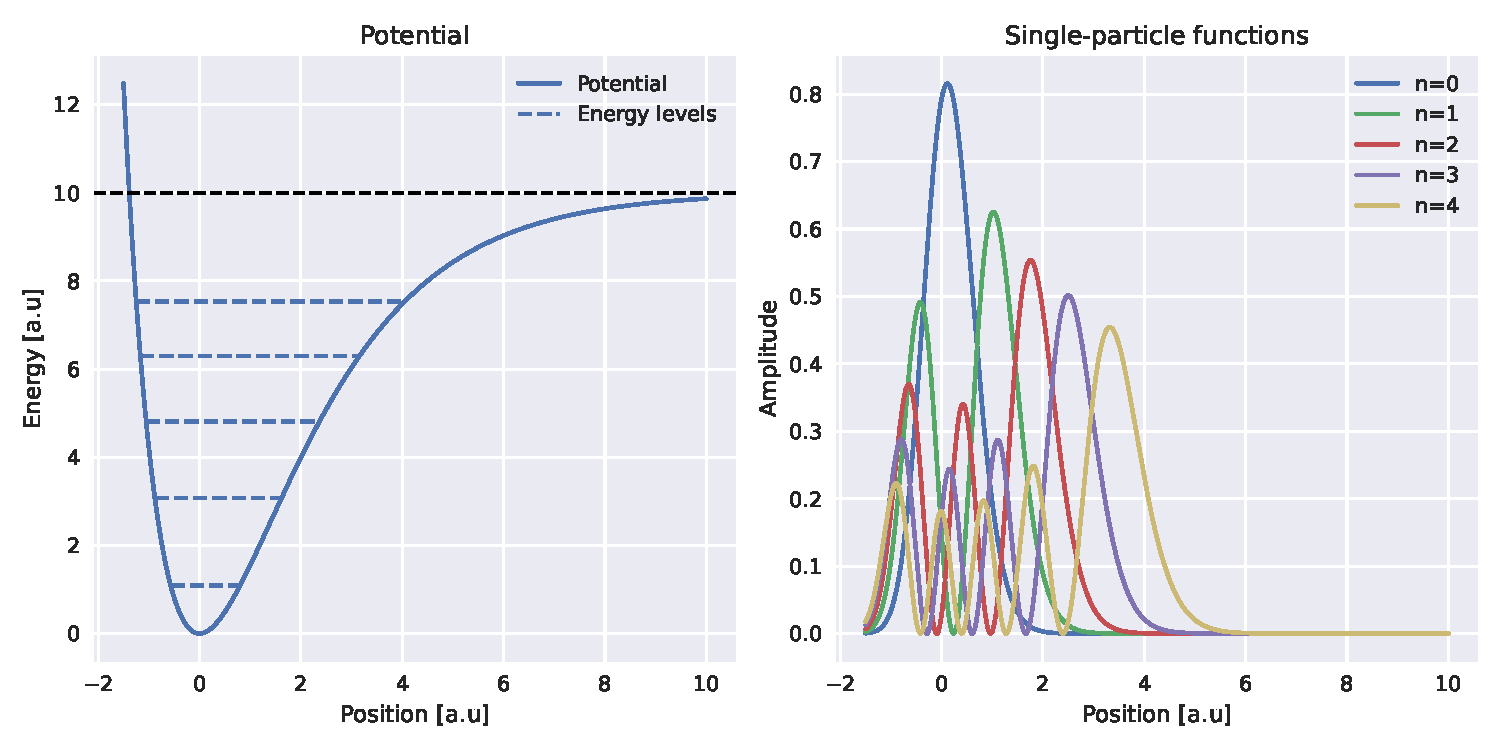
\includegraphics[width=0.8\textwidth]{figs/potential_spf.pdf}
    \caption{The Morse potential and the 5 lowest energy levels and energy eigenfunctions. The dissociation energy, $D$, is highlighted by the black dashed line. The parameters for this visualization of a Morse potential are $D=10, a=0.5, x_0=0$.}
    \label{fig:morse_potential}
\end{figure}


%% Double well
\\ \\Now, we would like to make a potential trap for \emph{two} separate particles, as our qubit system will be a two-particle system. To do so, we construct a double Morse potential well, simply by adding two Morse potentials together. We flip the right potential well, so that the minima are at the same position, and the potential is symmetric (given symmetric parameters). This gives us the double Morse potential as
\begin{equation}
    V(r) = D_L(e^{-c_L(r-r_{0,L})} - 1)^2 + D_R(e^{c_R(r-r_{0,R})} - 1)^2
\end{equation}
where the subscripts L and R correspond to left and right well, respectively. The parameter $D$ controls the depth of the potential well, whilst $c$ has some control over the width of the well, through the steepness of the exponential functions decay (and thus the curvature, and width, of the well). A smaller $c$ parameter constitues a wider well as the function would then decay slowly. The parameter $r_0$ is the position of the well minima. 

\begin{itemize}
    \item Presentation of the actual potential
    \item Why it is used, and where
    \item Connection to the long-range morse that is very popular
    \item Why we use it
    \item Form of the potential
    \item our construction of a double Morse potential well
    \item Some plots of the potential, and it's energy levels (show that they are quantized, but not equally spaced)
\end{itemize}

\subsection{Entanglement}
\begin{itemize}
    \item What is entanglement
    \item Why is it important
    \item How do we measure it
    \item How do we create it
    \item How do we use it - avoided crossings, ref \cite{nazir2005anticrossings}
\end{itemize}
\end{document}